\capitulo{3}{Conceptos teóricos}


Explicación de los conceptos teóricos básicos necesarios para que cualquier miembro del tribunal pueda entender el trabajo realizado.

Esta sección puede contener el número de subsecciones que sean necesarias.

\section{Sección}

\subsection{Subsección}

\subsubsection{Sub Subsección}

En esta sección y el resto de secciones de la memoria puede ser necesario incluir listas de items.

\begin{itemize}
    \item item1
    \item item2
    \item item3
    \item item4
\end{itemize}

Listas enumeradas.

\begin{enumerate}
    \item item1
    \item item2
    \item item3
\end{enumerate}

Figuras, como la figura \ref{fig:escudo} que aparece en la página \pageref{fig:escudo}. 

Puedes aprender más de las figuras en la dirección \url{https://es.overleaf.com/learn/latex/Inserting_Images}

\begin{figure}[h]
    \centering
    
\includegraphics[width=0.25\textwidth]{img/escudoSalud.pdf}
    \caption{Pie de la figura de la figura bla bla bla}
    \label{fig:escudo}
\end{figure}


También se pueden insertar tablas como \ref{tab:my-table}, que ha sido generada con \url{https://www.tablesgenerator.com/}.

\begin{table}[]
\begin{tabular}{lll}
a & b & c \\
1 & 2 & 3 \\
4 & 5 & 6
\end{tabular}
\caption{}
\label{tab:my-table}
\end{table}

Es necesario que todas las figuras y tablas aparezca referenciadas en el texto, como estos ejemplos.

Todos los conceptos teóricos deben de estar correctamente referenciados en la bibliografía. Por ejemplo, aquí estoy citando la página de \LaTeX{} de Wikipedia \cite{wiki:latex}.

También puede ser necesario utilizar notas al pie \footnote{como por ejemplo esta}, para aclarar algunos conceptos.


\section{Estado del arte y trabajos relacionados.}

Revisión bibliografica de que se está haciendo en la industria o la academia relativo al problema que se está tratando.

Enumeración y resumen de todos los trabajos relacionados de interés.

\section{LLM}
\subsection{Introducción a los modelos grandes de lenguaje}
\subsubsection{¿Qué es un LLM?}

Los Modelos de Lenguaje de Gran Escala (LLM) son sistemas de inteligencia artificial que se alimentan de enormes conjuntos de datos compuestos por billones de palabras en lenguaje natural. Este lenguaje natural es aquel que empleamos los seres humanos para comunicarnos, como por ejemplo el contenido en este trabajo. Estos datos pueden extraerse de diversas fuentes, como páginas web, artículos y documentos propios, dependiendo de la función que deseemos que el modelo desempeñe.

Estos modelos suelen basarse en redes neuronales que utilizan el aprendizaje profundo (Deep Learning) para descubrir las complejas relaciones entre las palabras presentes en los datos de entrenamiento. Este proceso puede requerir tanto una gran cantidad de tiempo como un potencial de computación que no está al alcance del usuario promedio, en la figura \ref{fig:graficallms} se puede apreciar la mucha diferencia que hay entre distintos modelos según su objetivo. Para esta investigación, se emplea el proceso de RAG (que será discutido más adelante) para enriquecer nuestros resultados.

\begin{figure}[h]
    \centering
    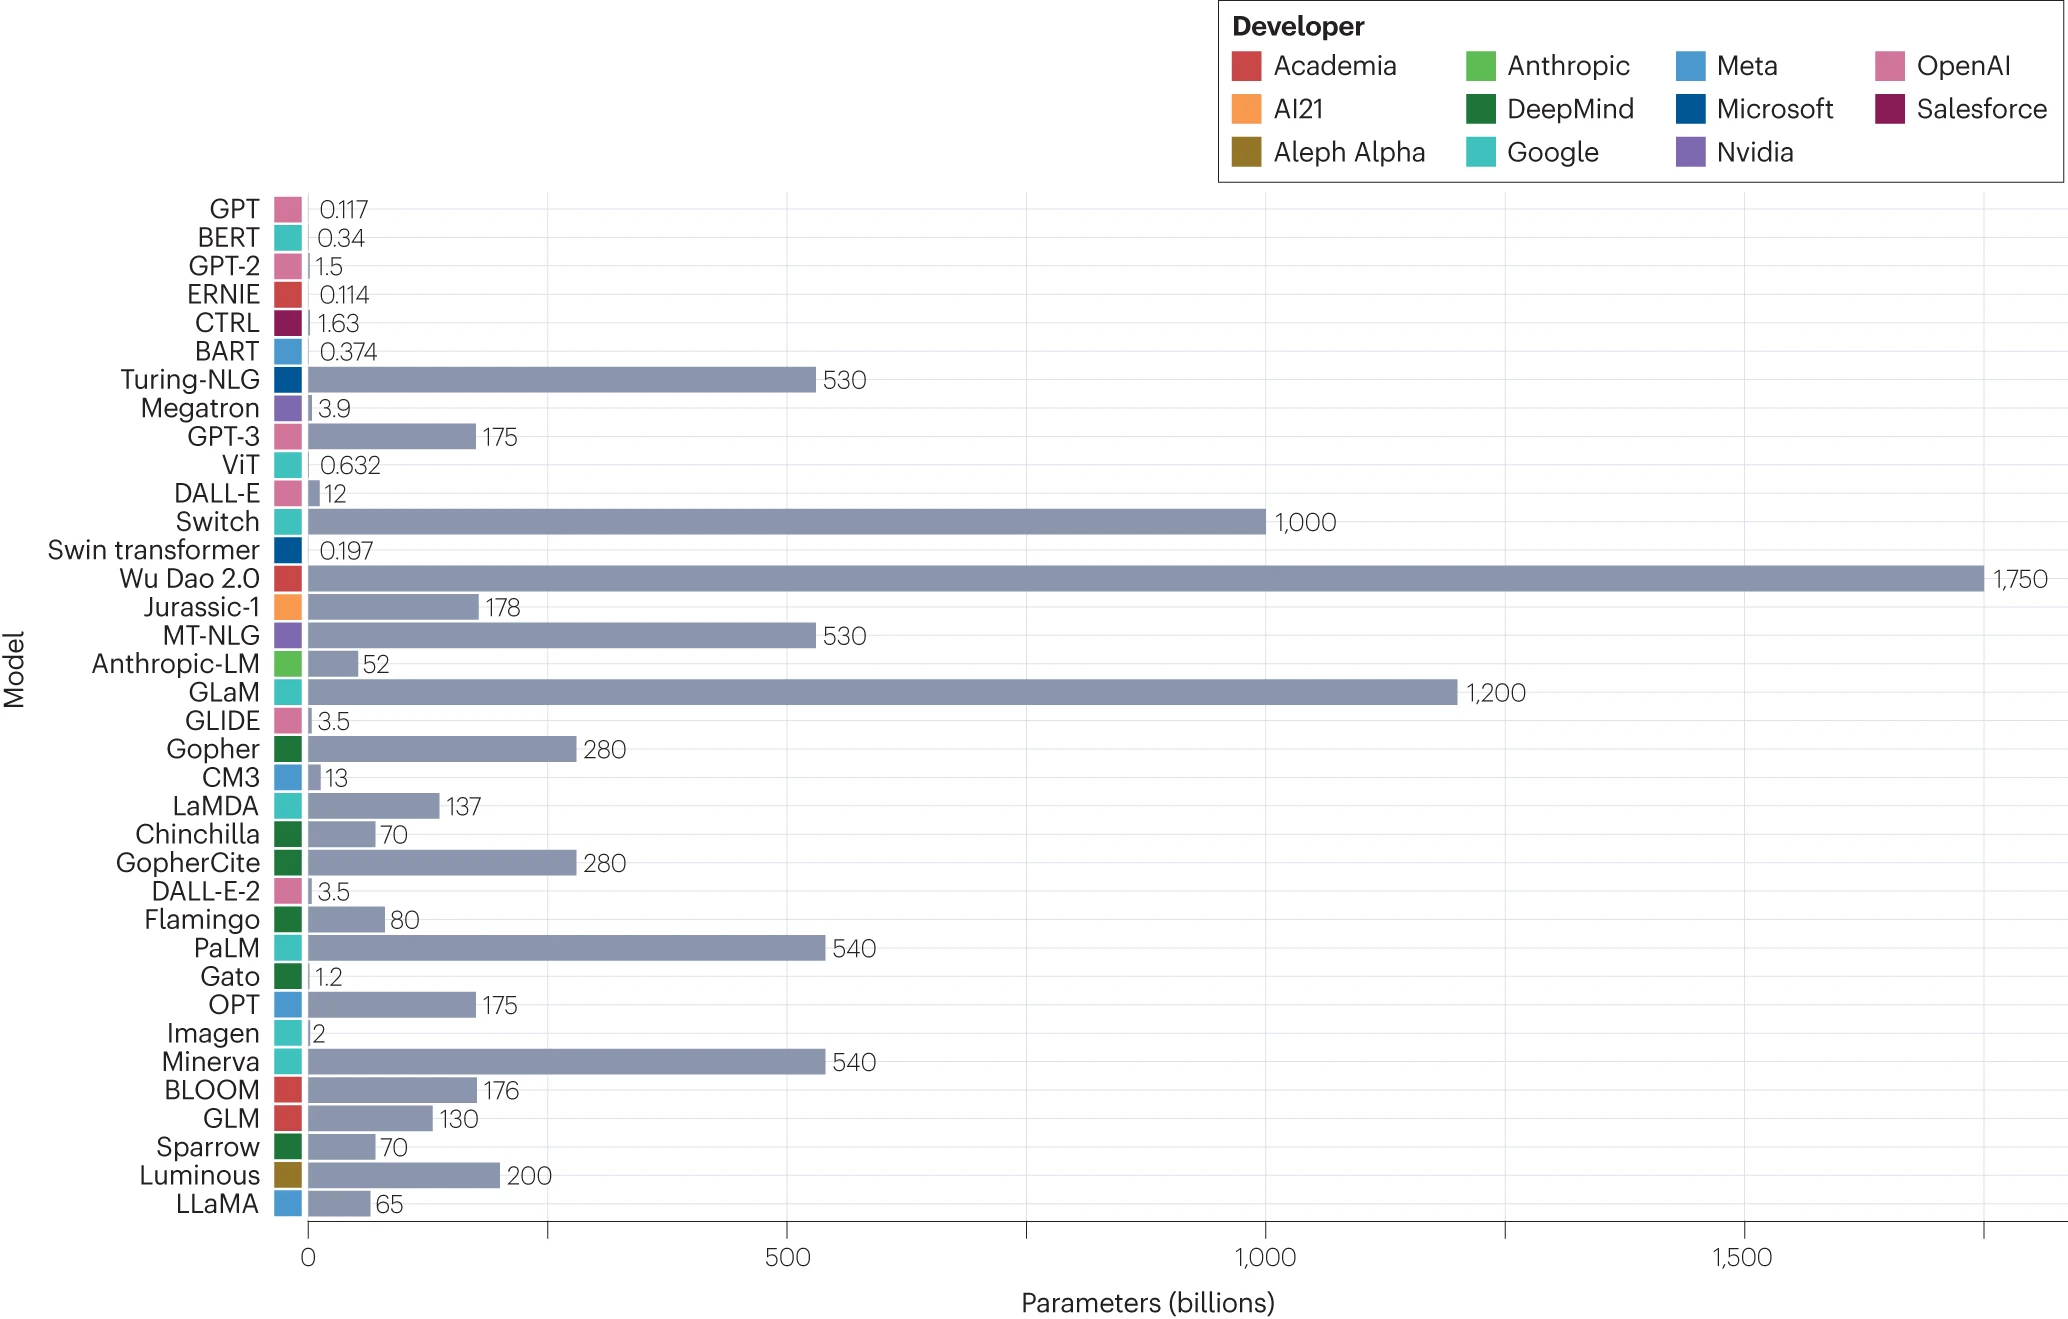
\includegraphics[width=1\textwidth]{img/recentllms.jpg}
    \caption{Comparativa de los billones de parámetros en distintos LLMs}
    \label{fig:graficallms}
\end{figure}

\subsubsection{Funcionamiento de los LLM}

Ahora que se ha hablado de que es un LLM procede explicar la tecnología que estos tienen por debajo, en esencia es lo que se conoce cómo transformadores, una tecnología presentada por Google en 2017. Esta tecnología resulto revolucionaria en el campo, dejando obsoleta rápidamente a los métodos que se empleaban para realizar predicciones en lenguaje natural antes de su aparición.

En esencia los transformadores se basan en la arquitectura codificador-decodificador en la que también se basan otras inteligencias artificiales, esta arquitectura consiste en, como su propio nombre indica, dos componentes principales, el codificador y el decodificador, en la figura \ref{fig:coddecod} se observa una representación de esta arquitectura. 

Un codificador no es más que un elemento matemático que convierte los datos de entrada en una representación matemática de los mismos, generalmente un vector, también llamada "hidden state". Por otra parte el decodificador recibe esa representación matemática de los datos de entrada y, según la tarea que se quiera realizar, traduce esa representación para ser parecida a aquella que fue introducida con el cambio deseado, como la traducción de un texto conservando su significado. En ambos elementos su funcionamiento depende enteramente de la tarea a realizar.

\begin{figure}[h]
    \centering
    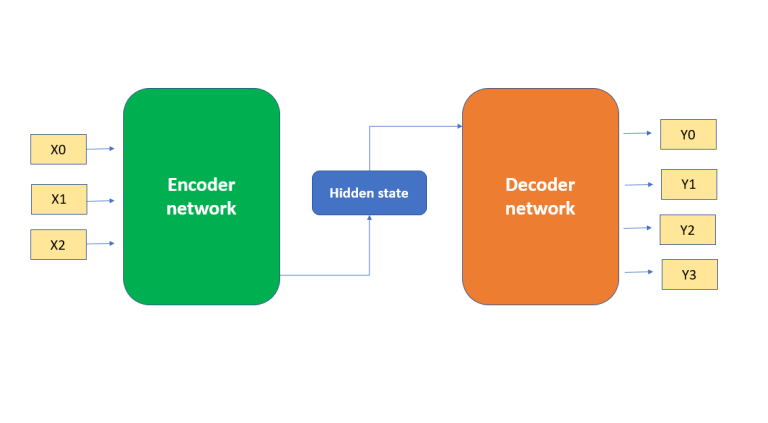
\includegraphics[width=1\textwidth]{img/encoder-decoder-architecture.png}
    \caption{Esquema de la arquitectura codificador-decodificador}
    \label{fig:coddecod}
\end{figure}

Los LLM por otra parte se basan en esta arquitectura, estos modelos funcionan mediante el proceso de embedding para ''entender'' las relaciones entre fragmentos de texto llamados tokens en la figura \ref{fig:llmarch} se puede ver un esquema del funcionamiento de la arquitectura subyacente a los LLMs.

Primero se debe dividir el texto de entrenamiento en fragmentos más pequeños (el tamaño de cada fragmento dependerá de la tarea) estos fragmentos serán los llamados tokens que son representados en el modelo por embeddings, un embedding es la representación vectorial del token en la que cada dimensión del vector representa un aspecto nuevo relacionado con el ámbito que está aprendiendo el modelo.

Este proceso de embedding tiene lugar en el codificador sin embargo esta forma de codificación resulta especialmente eficiente en grandes volúmenes de datos, prueba de ello es la gran mejora de rendimiento en LLMs con respecto a otros modelos de inteligencia artificial a la hora de realizar tareas con textos en lenguaje natural, dos vectores cercanos según técnicas matemáticas como la similitud del coseno o la distancia euclidiana se entienden cómo información relacionada para el LLM.

Cuando se genera una petición del usuario al modelo, se genera un embedding de la petición, los embeddings de los datos de entrenamiento más cercanos serán los que considere cómo posible respuesta.

Otro componente importante son los llamados mecanismos de atención, que capturan la información anterior y posterior al componente que se analiza para entender la información en su contexto y filtrar información poco relevante  manteniendo relaciones semánticas y contextuales entre palabras, otra ventaja importante a la hora de competir con otros modelos que no emplean estas tecnologías, estos mecanismos de atención se encuentran tanto en el codificador como en el decodificador.

\begin{figure}[h]
    \centering
    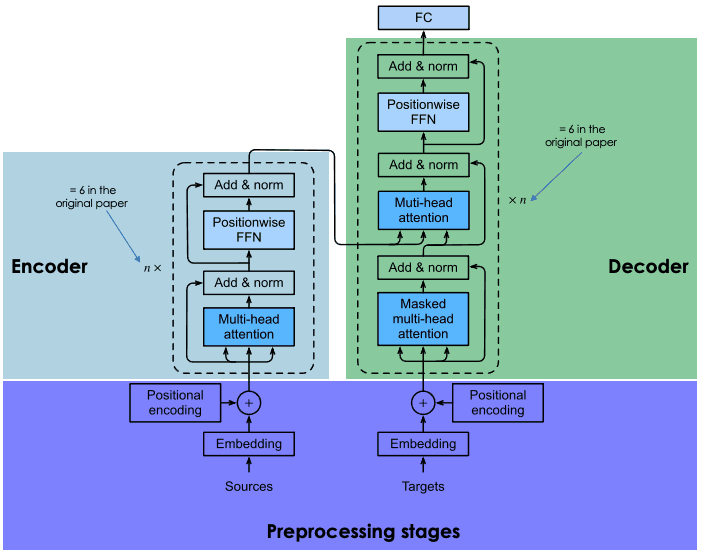
\includegraphics[width=1\textwidth]{img/llmarch.png}
    \caption{Esquema de la arquitectura de los transformadores en LLMs}
    \label{fig:llmarch}
\end{figure}

\subsection{Entrenamiento de LLMs}

Conociendo el funcionamiento subyacente a los LLMs es importante conocer ahora cómo estos modelos se entrenan ya que un modelo no entrenado no podría disponer de la información necesaria para aportarnos la información requerida.

El entrenamiento de un LLM cuenta de dos fases, el Pre-training y el Fine-tuning.

La fase de  pre-training es el paso inicial del entrenamiento, donde al modelo se le introduce una enorme cantidad de información en forma de tokens teniendo cómo objetivo que el modelo tenga un conocimiento general de la información proporcionada, este proceso es enormemente costoso en cuento a potencia de cálculo cómo en cuento a tiempo dependiendo de la magnitud del proyecto, esta etapa es, por lo tanto, la más costosa económicamente siendo este el motivo por lo que hay pocos modelos open-source ya que estos requieren una enorme inversión inicial.

El paso de fine-tuning consiste en obtener un modelo preentrenado (que haya pasado la fase de pre-training) y, por lo tanto, ya goce de un conocimiento general de las relaciones contextuales y semánticas de los datos de entrenamiento y ''ponerlo a punto'' especificando su conocimiento a datos más específicos, haciendo que funcione mejor en casos más concretos como, por ejemplo, los datos de una clínica especializada en cardiología. Esta mejora está más pensada cómo una forma de mejorar el conocimiento previo más que una manera de expandirlo.

En el estado del arte del entrenamiento en LLMs se encuentra, entre otras técnicas, el fine tuning, una metodología en la que el modelo ya entrenado ve, al igual que el fine-tuning, su rendimiento optimizado, esta vez siendo mejorado para que siga las instrucciones presentes en los prompts de manera más efectiva

\subsection{Parámetros de interés en un LLM}

Los parámetros en LLMs comprenden tanto la arquitectura del modelo, es decir, la programación subyacente que hace que todo funcione, el tamaño del modelo, los datos de entrenamiento y los hiperparámetros.
Los hiperparámetro en inteligencia artificial son variables de configuración del modelo empleadas para controlar el proceso de aprendizaje del mismo e influenciar en los resultados.
Los hiperparámetros importantes en LLMs comprenden la temperatura, top p, longitud del token, tokens máximos, tokens de parada entre muchos otros que escapan el alcance de este proyecto.

\subsubsection{Temperatura}

La temperatura controla la aleatoriedad de las respuestas del modelo, dicho con otras palabras, controla su creatividad a la hora de explorar respuestas, un modelo con una temperatura baja generará respuestas mas deterministas y fáciles de predecir siendo también más conservadoras con sus respuestas por lo que si se necesita una respuesta precisa con poca tolerancia a la creatividad y fallos es importante mantener una temperatura baja.

\subsubsection{Top-p}

El top-p, también conocido por nucleus sampling o muestreo de núcleo en español, es otro hiperparámetro que controla la aleatoriedad del modelo definiendo un límite que los tokens tienen que superar para ser considerados como respuesta del modelo, este último seleccionará aleatoriamente una respuesta de entre todas las que hayan superado el umbral seleccionado. 

\subsubsection{Longitud de token}

La longitud de token es simplemente el número de palabras o caracteres que componen los tokens con los que trabaja el modelo, este valor depende enteramente del propósito del modelo y de los datos de entrenamiento ya que una longitud de token muy pequeña puede hacer que se pierda contexto importante en la salida de los datos mientras que, por el contrario, tokens demasiado grandes harán que el modelo considere información poco relevante para la tarea que se espera que realice.

\subsubsection{Límite máximo de tokens}

El límite máximo de tokens es el número máximo de tokens que el modelo generará y procesará al mismo tiempo, cuanto mayor sea este máximo, más coherente será la salida, pero con el coste de ser también más computacionalmente costosa, este valor se definirá según el objetivo del modelo y de las limitaciones del hardware disponible.

\subsubsection{Tokens de parada}

Los tokens de parada son simplemente la longitud de la respuesta que el modelo diseñará, al igual que el límite de tokens un mayor valor supone un mayor coste computacional. Si este valor se fija en 1 la respuesta se limitará a una frase mientras que si aumenta a 2 esta consistirá en como mucho un párrafo.

\subsection{Prompts}
Un prompt es la manera que tiene el usuario para interactuar con el modelo mediante la creación de instrucciones en lenguaje natural que se le pasan al modelo para que tras los cálculos nos ofrezca e output deseado.

El output depende en gran parte del prompt así cómo de los datos de entrenamiento y los parámetros del modelo,que serán explicados posteriormente.

El Objetivo del prompt es aportar al modelo la información y el contexto necesario para que pueda ofrecer la respuesta deseada, las distintas técnicas para refinar un prompt que ofrezca el resultado deseado se las conoce como prompt engineering y en el siguiente apartado hablaremos más a fondo de ellas con un enfoque a su aplicación en la medicina y las ciencias de la salud.

\subsubsection{Prompt Engineering}

El Prompt Engineering es crucial a la hora de trabajar con modelos grandes de lenguaje y obtener los resultados deseados, en el ámbito sanitario un prompt puede definir escenarios reales y detallados con la mayor cantidad de información posible o especificando lo más concretamente posible la información que se quiera obtener de los datos de entrada .

Para reafirmar la potencia que tiene esta técnica en datos médicos, ChatGPT un chatbot que emplea un LLM consiguió mediante el uso de prompts adecuados llegar al nivel de aprobar el examen de licencia médica de Estados Unidos (USMLE) demostrando un gran nivel en sus razonamientos.

A la hora de diseñar prompts tenemos varios tipos los "Few-Shot" o los "Zero-shot" son dos de ellos. 

El Zero presente en el nombre quiere decir que el prompt será sobre un tema que nuestro modelo desconoce o posee poca información al respecto mientras que el shot indica que proporcionamos al LLM un ejemplo. Aunque esto en un primer vistazo parezca fútil o de poca utilidad pero este tipo de prompts resultan muy útiles para diversas tareas cómo la traducción de textos sin realizar ningun tratamiento o tarea específica al texto de entrada.

Los "Few-shot" prompts por su parte se diferencian de los "zero-shot" prompts en que contienen un ejemplo para ayudar al modelo a efectuar la tarea aunque tampoco sea la tarea aquella para la que el modelo haya sido entrenada.

Antes de hablar más a fondo de otros tipos de prompts es importante que se definan los niveles de complejidad que puede llegar a tener un prompt.

Los prompts de primer nivel simplemente consisten en preguntas muy simples sin refinar como por ejemplo, ¿Que es el Covid-19?
Los de Segundo nivel consisten en ofrecer un contexto al modelo para mejorar el prompt podría ser: Eres un profesor de ingeniería de la salud de la universidad de burgos y yo soy tu estudiante, ¿Me podrías enseñar sobre el Covid-19?
Por otra parte los de tercer nivel también agregan ejemplos a los mismos siguiendo la linea de los ejemplos podría consistir en aportar un abstract de un artículo relacionado con el Covid-19 y añadir el prompt de nivel 2 para obtener uno de nivel 3
Y, para finalizar los niveles, los de cuarto nivel permite al modelo descomponer la solicitud en componentes.

Otro método que ha probado obtener buenos resultados a la hora de crear prompts son los llamados prompts estructurados, estos consisten en aportar información extra en el prompt para dar forma a nuestro resultado deseado, hay muchas estrategias que ayudan a esto, suelen estar denominadas en siglas fáciles de recordar que indican de que información se compondrá nuestro prompt.

Las estrategias de prompts estructurados más conocidas son:

\begin{itemize}
    \item APE: Action, Purpose, Expectation
    \item RACE: Role, Action, Context, Expectation
    \item COAST: Context, Objective, Actions, Scenario, Task
    \item TAG: Task, Action, Goal
    \item RISE: Role, Input, Steps, Expectation
    \item TRACE: Task, Request, Action, Context, Example
    \item ERA: Expectation, Role, Action
    \item CARE: Context, Action, Result, Example
    \item ROSES: Role, Objective, Scenario, Expected Solution, Steps
    
\end{itemize}

Por último de hablará de los prompts iterativos, estos son aquellos que el propio LLM ayuda en su creación ya que se creará un prompt inicial y se le pedirá al modelo que vaya refinando el prompt, expresándole los deseos que quiere obtener, puede que se necesiten varias iteraciones para obtener un prompt lo suficientemente bueno y podría no ser una solución buena si se quiere realizar una búsqueda rápida pero ya que trabajamos con el propio modelo se podría asegurar un prompt de excelente calidad que obtenga información precisa y detallada que incluso puede superar las expectativas iniciales del usuario.

\subsubsection{Malos Prompts}

Se podrían considerar como malos prompts aquellos que no generen el resultado deseado o generan resultados de información falsa, cabe destacar que esto no siempre es culpa del prompt ya que un entrenamiento inadecuado puede conllevar al mismo resultado.

Malos prompts por lo general son aquellos poco preciosos o engañosos, un prompt poco preciso puede llevar al modelo a generar una respuesta poco precisa o generar una respuesta que no satisfaga al usuario ya que puede haber una cantidad insondable de información, por ejemplo, ¿Que enfermedad puede tener mi paciente? sin proporcionar más información, un modelo podría indicar que necesita más información o citar cierto número de enfermedades ya que estarán entre las posibles que pueda padecer.

Aquellos engañosos son en los que se introduce un sesgo como por ejemplo ¿Por qué los hospitales deberían aumentar el número de camillas? Cuando en realidad puede que la respuesta correcta sea que no deban hacerlo por los recursos de los que dispone al introducir el sesgo en la pregunta se pude recuperar respuestas engañosas. 

Otro tipo de prompts malos y engañosos son en los que se añade información falsa cómo por ejemplo ¿Que hongo causa el Covid-19? Aunque es cierto que muchos modelos detectan este error puede que un modelo más simple intente buscar alguna información que concuerde con el prompt.

\subsection{Usos comunes de los LLM}

En esta sección se expondrán áreas en las que los LLM podrían aportar información interesante, el campo de la medicina tendrá su propio apartado ya que, por el objetivo de la titulación y de este trabajo, es el campo que más interés posee por lo que se abordará en mayor profundidad.
\subsubsection{Ciberseguridad}

Un LLM puede ser entrenado con un gran volumen de datos de ciberseguridad cómo ataques pasados o consejos que publiquen expertos en el campo para poder predecir y anticiparse a futuros ataques, este campo resulta especialmente interesante debido al componente humano de los riesgos en linea ya que estos modelos analizan el lenguaje natural cómo ya se ha explicado con anterioridad. 
\subsubsection{Educación}

Los LLM se pueden emplear para diseñar material educativo personalizado para cada usuario, haciendo hincapié en los apartados en los que más fallos se cometan así cómo, empleando la función de memoria con la que cuentan muchas aplicaciones, hacer un seguimiento de la evolución del usuario.
\subsubsection{Atención al cliente}

Los LLM entrenados con la información de una empresa pueden ofrecer ayuda a las consultas que los clientes puedan tener sobre la misma así cómo ofrecer recomendaciones o consejos a estos mismos. Estas propiedades se pueden acentuar aún más empleando las técnicas de RAG.
\subsubsection{Traducción y localización}

Estos modelos también son potentes para salvar la barrera entre idiomas no sólo por ser capaz de traducir el texto, si no por ser capaz de localizarlo, es decir, adaptar el lenguaje para hacerlo más claro para el receptor que hable un idioma ajeno al original adaptando expresiones y modismos que pudieran resultar confusos si fuesen traducidos literalmente.
\subsubsection{Creación de contenido}

Otro campo en el que actualmente está destacando esta tecnología es en la creación de guiones iniciales, guías o bocetos para el desarrollo de libros, artículos, trabajos etc. Aunque el trabajo creativo siga estando de mano del usuario los LLM han probado ser una herramienta poderosa para guiar la creatividad del usuario y ayudarlo en la creación del producto final aumentando el rendimiento y la productividad.
\subsubsection{Análisis de datos}

En el campo del análisis de datos se destaca la capacidad de los modelos de generar información de los propios datos en diferentes formatos ya sea audio, vídeo o texto extrayendo la información relevante, generando resúmenes o respondiendo preguntas de la información contenida en los archivos de interés.

\subsection{Empleo de los LLMs en medicina}

El objetivo de este trabajo es dar una demostración de una posible aplicación de esta herramienta tan potente a un campo tan crucial para la sociedad como es la medicina y aunque la aplicación propuesta ya es en si misma un ejemplo de esto no está limitado a ello y en esta sección se explorarán mas aplicaciones y avances.
En primer lugar tenemos el procesado de lenguaje natural más convencional a la hora de interpretar datos y emitir diagnósticos y es que una versión del modelo PaLM 2 de Google aplicada a la medicina conocida como Med-PaLM 2 ha conseguido funcionar a un altísimo nivel, siendo equiparado al nivel de un clínico experto incluso en algunos casos llegando a superarlos en campos como la empatía con el paciente.

Aunque la información anterior da la visión de que la inteligencia artificial puede sustituir a los médicos profesionales a la hora de emitir un diagnóstico esto no es así ya que hay campos con menos estudios relacionados los cuales hace que los modelos den datos incompletos o directamente perjudiciales para el paciente ya que intenta ofrecer una respuesta aunque no la tenga cuando en ese caso un médico conduciría otras pruebas o solicitaría una segunda opinión por lo que los LLM aunque todavía no puedan sustituir a un médico especialista si ayudan a agilizar el proceso de diagnóstico y, por lo tanto, aumentan la eficiencia del sistema de salud.

Otro campo en el que los LLM parecen hacerse hueco en el mundo de la medicina es en la gestión de los recursos hospitalarios, el uso de camas, la medicina de triaje etc ofreciendo soluciones rápidas y efectivas cuando más se necesita siempre que esté alimentado con los datos de los recursos de los que el hospital dispone.

Otro posible avance que puede suponer la implementación de tecnologías de chatbots especializados en medicina puede ser la implementación de asistencia médica. Aunque este campo requiera mucha información ya que en la actualidad dejar a un modelo grande de lenguaje decidir un tratamiento o proveer asistencia médica a enfermos puede ser peligroso por las limitaciones actuales, se abre un campo de estudio muy interesante, el desarrollo de asistentes médicos virtuales entrenados en datos especializados los cuales, mediante el proceso de RAG, pueden incluir los datos específicos del paciente en cuestión, proporcionando ayuda especializada y revisada por profesionales médicos aliviando la carga de muchos profesionales médicos solventando posibles problemas de colapsos en la sanidad que tan graves resultan en la actualidad, esto podría haber sido una gran ayuda en la época de la pandemia y merece la pena investigar en ello por posibles situaciones similares en un futuro.


\subsection{Desventajas y malos usos de los LLMs}

Aunque los LLM tengan grandes ventajas en su condición cómo herramientas viene implícita los malos usos que los usuarios les pueden dar ya no hablando de generar un prompt malo o insuficiente que genere resultados indeseados o pobres, si no de directamente emplearlos para actividades inmorales como el plagio y es que, cómo se ve en la figura \ref{fig:prosandcons}, aunque los beneficios superan en enorme medida los riesgos ignorarlos sería caer en un error grave así cómo lo sería obviar los grandes avances que esta tecnología está generando y promete generar en un futuro.

\begin{figure}[h]
    \centering
    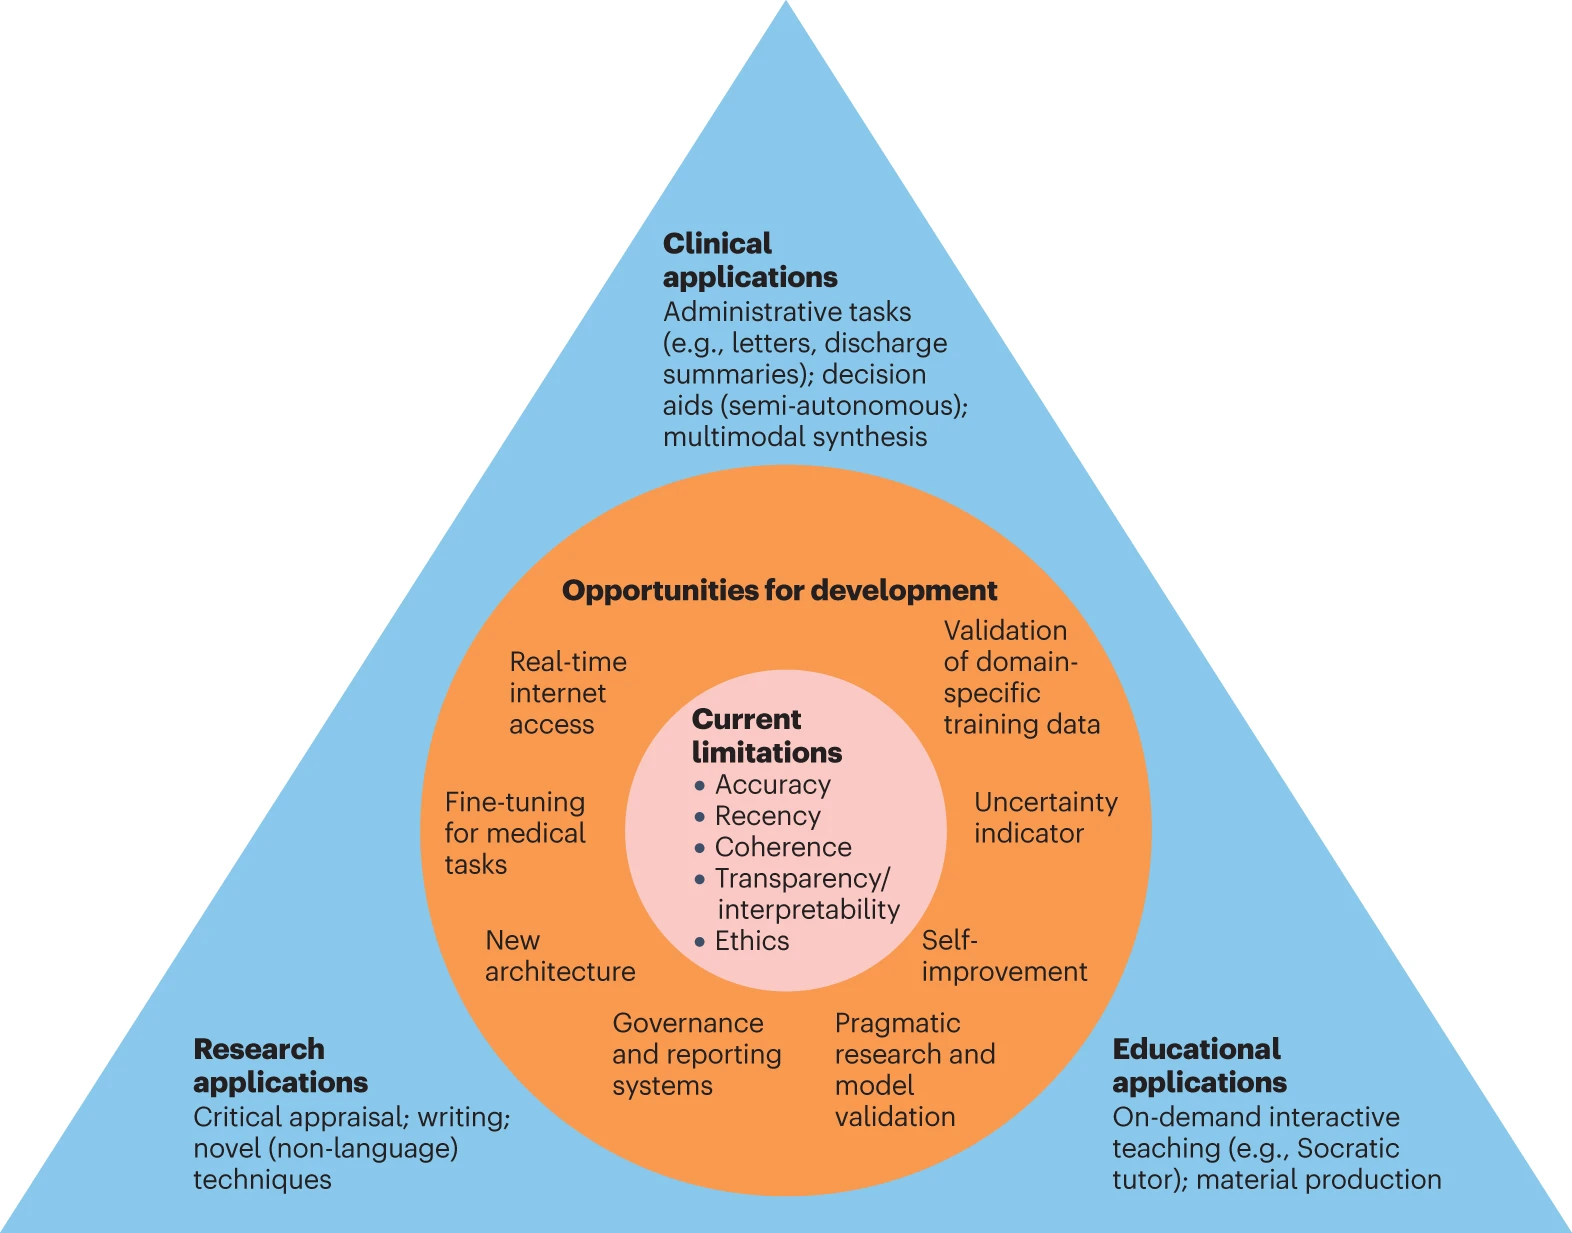
\includegraphics[width=1\textwidth]{img/pros_and_cons.jpg}
    \caption{Algunos beneficios y limitaciones de los LLM}
    \label{fig:prosandcons}
\end{figure}

\subsection{Diferentes LLMs}

Actualmente y al ser una tecnología nueva, revolucionaria y que está demostrando grandes resultados, hay multitud de modelos, se hará un repaso de los más influyentes. En la tabla \ref{tab:tablellm} se puede consultar información relevante de los mismos.

\begin{table}[]
\begin{tabular}{lllll}
\textbf{Nombre del Modelo}     & \textbf{Desarrolladora}                & \textbf{Acceso}           &  &  \\
GPT                     & OpenAI                          & API              &  &  \\
Gemini                  & Google                          & API              &  &  \\
Gemma                   & Google                          & Open             &  &  \\
Llama 3                 & Meta                            & Open             &  &  \\
Vicuna                  & LMSYS Org                       & Open             &  &  \\
Claude 3                & Anthropic                       & API              &  &  \\
Stable Beluga           & Stability AI                    & Open             &  &  \\
StableLM 2              & StabilityAI                     & Open             &  &  \\
Coral                   & Cohere                          & API              &  &  \\
Falcon                  & Technology Innovation Institute & Open             &  &  \\
DBRX                    & Databricks and Mosaic           & Open             &  &  \\
Mistral 8x7B and  8x22B & Mistral AI                      & Open             &  &  \\
XGen-7B                 & Salesforce                      & Open             &  &  \\
Grok                    & xAI                             & Chatbot and Open &  & 
\end{tabular}
\caption{Principales LLMs en la actualidad}
\label{tab:tablellm}
\end{table}

\subsubsection{GPT – OpenAi}

Posiblemente el modelo más reconocido a día de hoy, presente en una aplicación que se ha vuelto de uso casi rutinario, ChatGPT, su nombre proviene de las siglas de Generative Pre-trained Transformer, cuenta con más de 175 mil millones de parámetros en su versión GPT-3 los cuales aumentan en sus versiones posteriores, GPT-3 Turbo, GPT-4 y GPT-4 Turbo, en la actualidad muchas empresas emplean sus servicios como por ejemplo Microsoft o la app de idiomas Duolingo.

\subsubsection{Gemini- Google}

 De menos parámetros, unos 3 mil millones está diseñado para operar en distintos dispositivos y con diferentes tipos de inputs ya sean estos audio, texto vídeos o código. Actualmente su uso principal reside en las aplicaciones de Google
 
\subsubsection{Llama 3 – Meta}

EL modelo de la gigante tecnológica meta destaca por tener, actualmente en entrenamiento, un modelo de 400 mil millones de parámetros, una cantidad insondable para muchas empresas, aparte de tener dos opciones más pequeñas de 70 y 8 mil millones de parámetros y también por ser de código abierto para usos comerciales y de investigación, por lo que muchos modelos aquí listados usan Llama 3 cómo su base.

\subsubsection{Mistral – Mistral}

Sus modelos destacan por su relativamente pequeño tamaño y por la optimización que estos tienen lo cual les permite rivalizar a otros modelos más grandes y usados por grandes empresas, esta optimización de parámetros le permite al modelo ejecutarse más rápido y en un hardware mucho menos potente que sus competidores.


\section{proceso de RAG}
\subsection{Introducción al RAG}

Al trabajar con modelos grandes de lenguaje, muchas veces la respuesta que se obtiene denotan la falta de información que estos modelos poseen sobre los datos ya que sólo entienden las relaciones entre tokens por lo que para aumentar la calidad de nuestros resultados se ha implementado un framework llamado RAG (Retrieval Augmented Generation) para aumentar y acotar, con los recursos ya existentes del modelo, la información que posee alimentándolo con los datos que puedan resultar de interés para la tarea.

El principal beneficio de emplear técnicas de RAG en LLMs consiste en poder realizar consultas precisas a los datos aportados por el usuario, esto en empresas cómo en sectores sanitarios es muy útil ya que si el repositorio de información empleada para el proceso de RAG es una base de datos, podríamos interactuar con ellos en tiempo real realizando tareas habituales de LLMs cómo consultas de forma cómoda y en lenguaje natural por lo que todo profesional sanitario con mínimos conocimientos informáticos podría interactuar con la base de datos de manera precisa y sin riesgos de que tome información de recursos poco fiables o que no tengan que ver con la tarea a realizar.

En la figura \ref{fig:ragrpoc} se puede ver una representación gráfica del proceso de RAG

\begin{figure}[h]
    \centering
    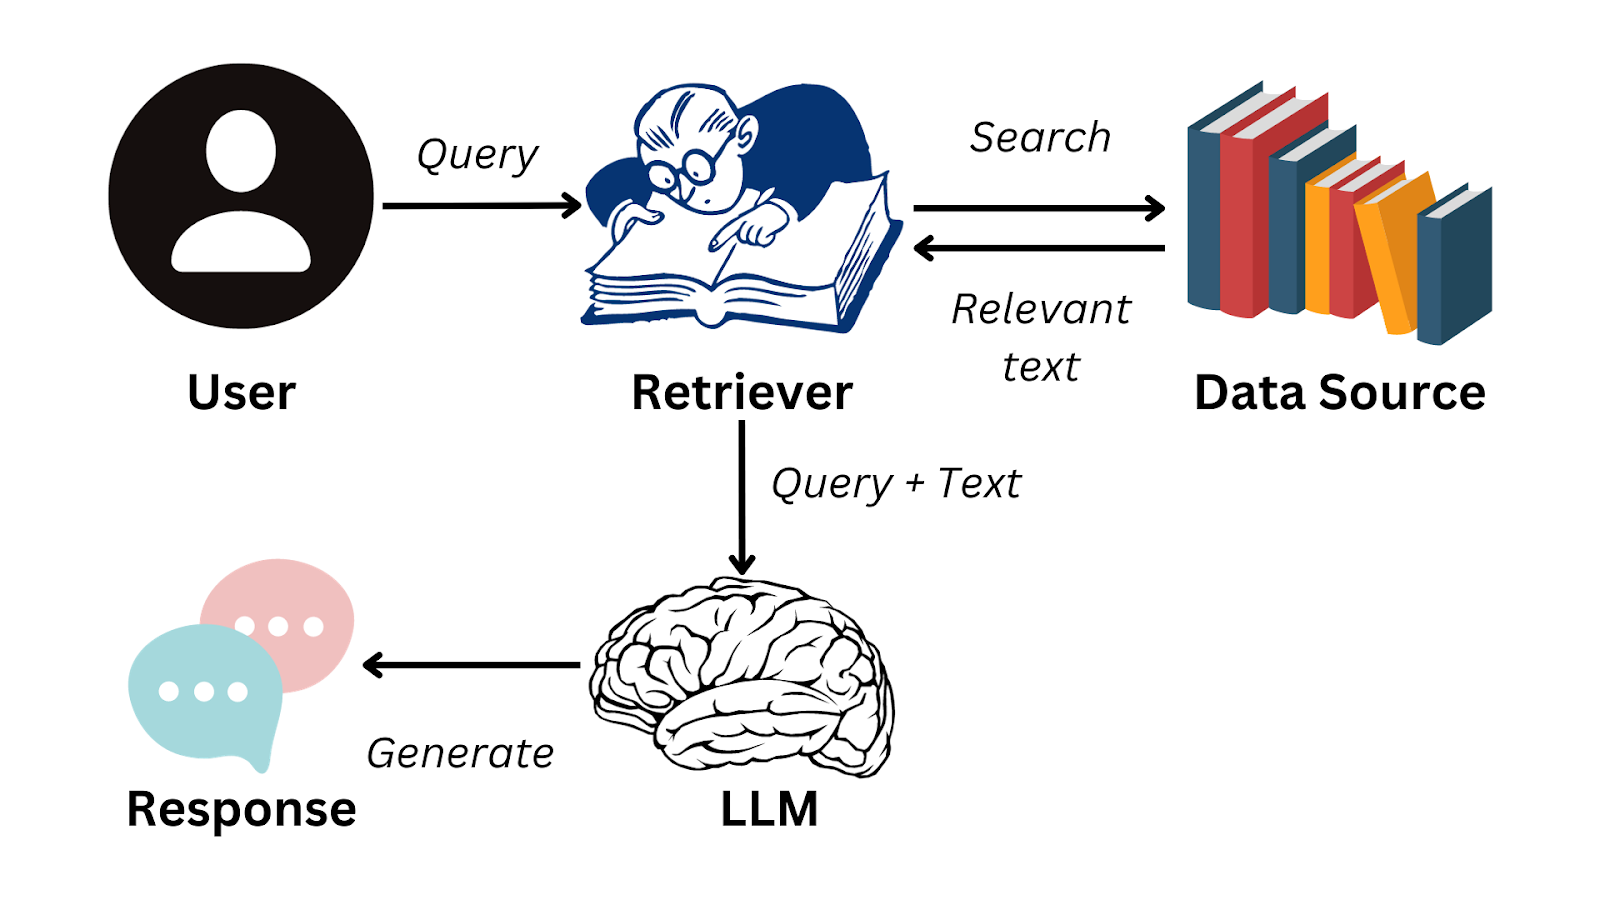
\includegraphics[width=1\textwidth]{img/ragproc.png}
    \caption{Proceso de RAG}
    \label{fig:ragrpoc}
\end{figure}


\subsubsection{Descripción del proceso de RAG}

El primer paso, evidentemente, consiste en identificar en que datos se quiere que se especialice el modelo y recuperarlos, el formato puede ser muy diverso, desde vídeos, CSV, PDFs, páginas web, bases de datos etc.

Seguido, se debe realizar un proceso similar al descrito en el apartado de entrenamiento de modelos, dividir la información de interés en chunks (trozos) que contengan diferente información relacionada para aumentar la eficiencia sin procesar documentos enteros y una vez obtenidos habrá que hacerlos pasar por el proceso de embedding, generando embeddings por cada chunk.

Una vez realizado los embeddings de los datos de interés hay que esperar a la petición del usuario y generar un embedding de esta última también, una vez generado se comparan las distancias entre el embedding de la petición y se devuelven los embeddings de los chunks más cercanos junto a los de la petición.

Y por último, teniendo los chunks relevantes a la petición junto a la misma, se insertan ambos en un LLM que generará una respuesta empleando la petición junto a los datos relevantes a la misma.

\section{PubMed}

PubMed es una página web gratuita fundada en 1996, contiene abstracts de  literatura biomédica así cómo los enlaces para recuperar los textos completos, varios de los artículos empleados para la elaboración de este trabajo así como los abstracts empleados para el proceso de RAG de la aplicación han sido recuperados de PubMed.

Los recursos de PubMed tienen varios orígenes.

\subsection{MEDLINE}

El componente principal de PubMed, la literatura científica aquí presente consiste en citas de revistas científicas indexadas con MeSH, unos términos especiales para facilitar la navegación en literatura biomédica.

\subsection{PubMed Central}

El segundo componente de PubMed, contiene artículos completos de revistas científicas revisados y seleccionados por la Biblioteca Nacional de Medicina (NLM)
\subsection{Bookshelf}

El componente final de PubMed, contiene libros, informes, bases de datos y otros documentos relacionados con la biomedicina.

\section{COVID-19}

El COVID-19 es un virus causante del síndrome agudo respiratorio severo, que originó una pandemia declarada cómo tal el 11 de Marzo por la Organización Mundial de la Salud (OMS), por el peligro inminente que supuso y el impacto mundial que causó, generó en la época de pandemia y posteriormente, una gran cantidad de datos.